\documentclass[12pt,letterpaper]{article}

% just for the example
\usepackage{lipsum}
% Set margins to 1.5in
\usepackage[margin=1.5in]{geometry}

% for graphics
\usepackage{graphicx}
\graphicspath{{./figures/p3/}}

% for crimson text
\usepackage{crimson}
\usepackage[T1]{fontenc}

% setup parameter indentation
\setlength{\parindent}{0pt}
\setlength{\parskip}{6pt}

% for 1.15 spacing between text
\renewcommand{\baselinestretch}{1.15}

% For defining spacing between headers
\usepackage{titlesec}
% Level 1
\titleformat{\section}
  {\normalfont\fontsize{18}{0}\bfseries}{\thesection}{1em}{}
% Level 2
\titleformat{\subsection}
  {\normalfont\fontsize{14}{0}\bfseries}{\thesection}{1em}{}
% Level 3
\titleformat{\subsubsection}
  {\normalfont\fontsize{12}{0}\bfseries}{\thesection}{1em}{}
% Level 4
\titleformat{\paragraph}
  {\normalfont\fontsize{12}{0}\bfseries\itshape}{\theparagraph}{1em}{}
% Level 5
\titleformat{\subparagraph}
  {\normalfont\fontsize{12}{0}\itshape}{\theparagraph}{1em}{}
% Level 6
\makeatletter
\newcounter{subsubparagraph}[subparagraph]
\renewcommand\thesubsubparagraph{%
  \thesubparagraph.\@arabic\c@subsubparagraph}
\newcommand\subsubparagraph{%
  \@startsection{subsubparagraph}    % counter
    {6}                              % level
    {\parindent}                     % indent
    {12pt} % beforeskip
    {6pt}                           % afterskip
    {\normalfont\fontsize{12}{0}}}
\newcommand\l@subsubparagraph{\@dottedtocline{6}{10em}{5em}}
\newcommand{\subsubparagraphmark}[1]{}
\makeatother
\titlespacing*{\section}{0pt}{12pt}{6pt}
\titlespacing*{\subsection}{0pt}{12pt}{6pt}
\titlespacing*{\subsubsection}{0pt}{12pt}{6pt}
\titlespacing*{\paragraph}{0pt}{12pt}{6pt}
\titlespacing*{\subparagraph}{0pt}{12pt}{6pt}
\titlespacing*{\subsubparagraph}{0pt}{12pt}{6pt}

% Set caption to correct size and location
\usepackage[tableposition=top, figureposition=bottom, font=footnotesize, labelfont=bf]{caption}

% set page number location
\usepackage{fancyhdr}
\fancyhf{} % clear all header and footers
\renewcommand{\headrulewidth}{0pt} % remove the header rule
\rhead{\thepage}
\pagestyle{fancy}

% Overwrite Title
\makeatletter
\renewcommand{\maketitle}{\bgroup
   \begin{center}
   \textbf{{\fontsize{18pt}{20}\selectfont \@title}}\\
   \vspace{10pt}
   {\fontsize{12pt}{0}\selectfont \@author} 
   \end{center}
}
\makeatother

% Used for Tables and Figures
\usepackage{float}

% For using lists
\usepackage{enumitem}

% For using APA Citation format
\usepackage{apacite}

% Custom Quote
\newenvironment{myquote}[1]%
  {\list{}{\leftmargin=#1\rightmargin=#1}\item[]}%
  {\endlist}
  
% Create Abstract 
\renewenvironment{abstract}
{\vspace*{-.5in}\fontsize{12pt}{12}\begin{myquote}{.5in}
\noindent \par{\bfseries \abstractname.}}
{\medskip\noindent
\end{myquote}
}

\begin{document}

% Set Title, Author, and email
\title{Assignment P3}
\author{Snejana Shegheva \\ sshegheva3@gatech.edu}

\maketitle
\thispagestyle{fancy}

\subsection*{Question 1 - Design Principles and Heuristics}

\subsection*{Question 2 - Constraint, Mappings and Affordances Principles}

Although, not entirely an activity of my everyday life, I used to regularly participate in an adrenaline-raising practice of flying trapeze. For safety reasons, all students must wear belt harness. When on the platform, safety lines are attached to the belt so that a trained professional can reduce the impact of wrong falling. Figure~\ref{fig::1} demonstrates attaching a carabiner (that holds safety lines) to a belt in two ways: \textit{overhook} vs \textit{underhook}\footnote{The terms \textit{overhook} vs. \textit{underhook} in this context have nothing to do with wrestling}. The preferred way is to use \textit{overhook} position that greatly simplifies the process of detachment. Although the \textit{underhook} position is not wrong, it makes it very inconvenient for your wrists to twist the lock to open and release. It is very \textbf{easy} to hook the carabiners from savety lines to the belt harness in the sub-optimal way because there is nothing to prevent you from hooking it in either direction (and both do their job of protecting you from a fall). The \textbf{penalty} here comes \textit{after} completing the jump where you have to release the safety lines from both your sides. It takes a lot of wiggling the carabiners around to put them back in the position where it is possible to unlock them safely for subsequent transfer back to the person on the board.   

\begin{figure}[h]
\centering
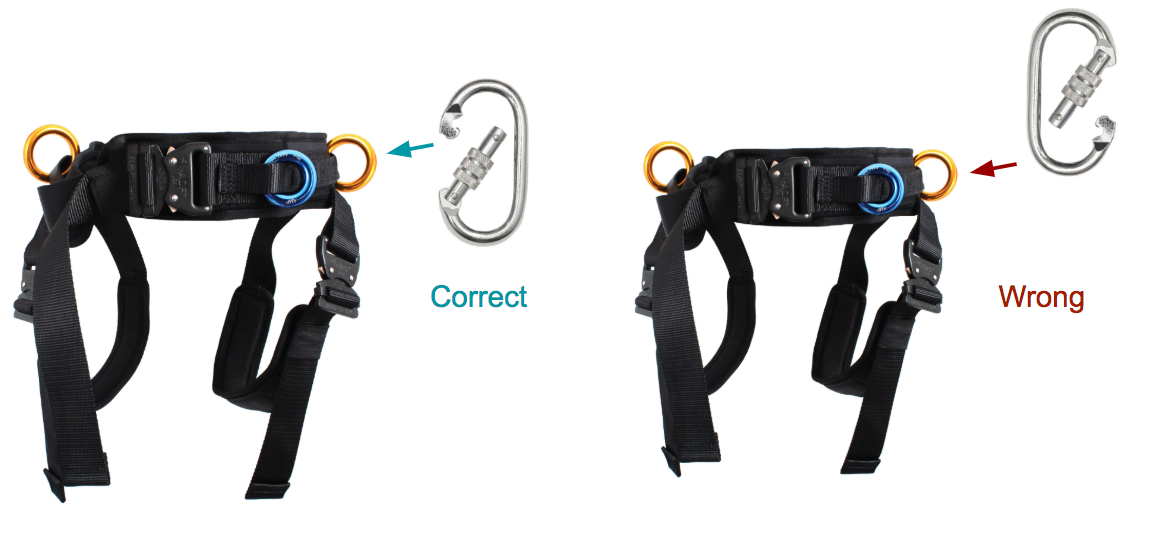
\includegraphics[width=3in,scale=.5]{figures/p3/flying_trapeze.png}
\caption{Demonstration of two ways to attach a carabiner to a belt. Left: preferred. Right: Inconvenient (especially for detaching using one hand.)}
\label{fig::1}
\end{figure}

\subsubsection*{Constraints}
One clue for limiting the wrong action is to modify the ring on the belt that constrains you from passing the hook unless it is a specific position. For example, changing the thickness of the rings in different areas can guide the proper clasping position. Alternatively, the hook on the carabiner itself can have a more intricate shape that forces you to angle it in a certain way.

\subsubsection*{Mappings}
Don Norman defines a  \textit{mappings} design principle in terms of relationship a control and resulting function\cite{norman2013design}. The result of a carabiner locking depends on how the person originally holds it. Therefore, a mapping principle suggests to add visual clues for desired alignment between the hand and the carabiner. Similarly to how some shipping packages are labeled with an arrow pointing up, the surface of the carabiner can be engraved with an arrow to hint on the direction of hold.    

\subsubsection*{Affordances}
A strong relative to mapping principle is \textit{affordance} principle that determines the interaction method between the agent and the interface \cite{norman2013design}. To improve the carabiner interface, its shape can be mapped to the shape of the palm. When we clasp our hands, it is more natural the grip to be wider closer to the thumb, and more narrow towards the pinkie. If the carabiner for flying trapeze can resemble a \textit{pear} shape, it would be more intuitive to grasp the carabiner in a certain way that it more likely for you to hook it from a right angle. The shape in this case affords a proper handle \textit{before} the carabiner is attached.


\subsection*{Question 3 - Slips, Mistakes and Errors}

Yousician 

Slip: missing a note 
Mistake: Hitting an incorrect note (ex, missing sharps in G major)

First, describe a slip that a player of the game might make. Remember, a slip generally occurs when the player knows what action they should take, but does something different instead. In Tetris, this might be a player wanting to move a piece to the right, but pressing the left button instead. Then, describe why the player might make that slip. Then, briefly suggest a way the interface could be changed to prevent that slip in the future.

Second, describe a mistake that a player of the game might make. Remember, a mistake generally occurs when the player knows what they want to accomplish, but doesn’t know how to actually make it happen. In Tetris, this might be a player wanting to rotate a piece clockwise, but pressing to rotate it counter-clockwise instead because they do not know which button rotates clockwise. Then, describe why the player might make that mistake. Then, briefly suggest a way the interface could be changed to prevent that mistake in the future.

Finally, describe something that makes the game challenging, but that is not a slip or a mistake. For example, in Tetris, there may be no obvious place for a piece to go, but that does not force the user to commit a slip or a mistake.

\subsection*{Question 4 - Representation of the underlying content}

\bibliographystyle{apacite} 
\bibliography{bibtemp}

\end{document}
